\documentclass[a4paper, 12pt]{scrartcl}
\usepackage{scrpage2}
\usepackage[left=2.5cm,right=2.5cm, top=3cm, bottom=4cm]{geometry}
\usepackage[utf8]{inputenc}
\usepackage[ngerman]{babel}
\usepackage[T1]{fontenc}
\usepackage{amsmath}
\usepackage{amssymb}
\usepackage{amsfonts}

\usepackage{graphicx}

\usepackage{float}
\usepackage{adjustbox}
\usepackage{hyperref}
\usepackage{textcomp}
\usepackage{multirow}
\usepackage{array}

%\usepackage{enumerate}
\usepackage[shortlabels]{enumitem}

%Zeichnungen
\usepackage{tikz}
\usepackage[european]{circuitikz}

% Einrücken verhindern
\setlength{\parindent}{0em} 


\begin{document}

\begin{titlepage}
	\centering
	{\Huge\bfseries Versuchsprotokoll\par}
	\vspace{2cm}
	{\scshape\LARGE Elektrizitätslehre \par}
	\vspace{1cm}
	{\Large Gedämpfter LCR-Schwingkreis und \\ Gekoppelte LC-Schwingkreise\par}
	\vfill
	{\large\itshape Simon Schwarz und Marius Ising\par}

	\vfill
\end{titlepage}

\tableofcontents
\newpage


\section{Gedämpfter LCR-Schwingkreis}


\subsection{Versuchsbeschreibung}

In einer Serienschaltung aus Spule $L$, Kondensator $C$ und Ohmschem Widerstand $R$ (vgl. Abb. \ref{abb:schaltLCR}) wird der Kondensator zunächst aufgeladen und anschließend die Spannungsquelle mit einem Taster überbrückt, sodass der Kondensator sich über den Widerstand entladen kann. Dabei entlädt sich der Kondensator nicht sofort, sondern er schwingt sich bei der Spannung $U=0$ ein. Dieser Einschwingvorgang hängt wesentlich von der Dämpfung der Schwingung durch die Ohmschen Widerstände der Schaltung ab.

\begin{figure}[H]
\centering
\begin{tikzpicture}
\draw (2,0) node[ocirc]{} -- (2,1) to [C, a=$C$] (2,3) to [R, a=$R$] (4,3)  to [cute inductor, a=$L$] (6,3) to[rmeterwa, t=$I$] (6,1) -- (6,0) node[ocirc]{};
\draw (2,1) to [push button] (6,1);
\draw (2,1.2) -- (1,1.2) to [rmeterwa, t=$U_C$] (1,2.8) -- (2,2.8);
\end{tikzpicture}
\caption{Schaltbild des LCR-Schwingkreises}
\label{abb:schaltLCR}
\end{figure}

Nach der Kirchhoffschen Maschenregel gilt für die Schaltung bei gedrücktem Taster
$$0 = U_C + U_R + U_L = \frac QC + RI + L \frac{dI}{dt}$$
Mit $I = \frac{dQ}{dt}$ erhält man folgende Differentialgleichung
$$\frac{d^2Q}{dt^2} + \frac{R}{L} \frac{dQ}{dt} + \frac{1}{LC}Q = 0$$
Dies ist die DGL einer gedämpften harmonischen Schwingung. Dabei bezeichnet $\delta = \frac{R}{2L}$ die Dämpfungskonstante und $\omega_0 = \frac{1}{\sqrt{LC}}$ die Schwingungsfrequenz der ungedämpften Schwingung. 
Für die Lösung der DGL unterscheiden wir drei Fälle. In allen Fällen gelten die gleichen Anfangsbedingungen
$$Q(0) = CU_0 \hspace{0.5cm} \text{ und } \hspace{0.5cm} I(0) = 0.$$

\textbf{Schwingfall ($\delta < \omega_0$)} \\
Hier ist eine echte Schwingung zu beobachten. Es gilt
$$Q(t) = e^{-\delta t}( A\cos(\omega t) + B\sin(\omega t)).$$
Aus den Anfangsbedingungen erhält man $A = CU_0$ und $B = A \frac{\delta}{\omega}$. Für den Strom gilt wegen $I = \frac{dQ}{dt}$
\begin{equation}\label{eq:i_lsg}
I(t) = -CU_0 e^{-\delta t} \left( \omega + \frac{\delta^2}{\omega}\right)\sin(\omega t)\text{.}
\end{equation}

\textbf{Kriechfall ($\delta > \omega_0$)} \\ 
In diesem Fall ist die Dämpfung so stark, dass der Kondensator seine Spannung nur sehr langsam verliert. Zudem findet keine Schwingung statt.
$$Q(t) = Ae^{\left( -\delta + \sqrt{\delta^2-\omega_0^2} \right)t} + Be^{\left(-\delta - \sqrt{\delta^2-\omega_0^2} \right)t}$$
Aus den Anfangsbedingungen ergibt sich
$$A = CU_0 \frac{\delta +\sqrt{\delta^2-\omega_0^2}}{2\sqrt{\delta^2-\omega_0^2}} \hspace{0.5cm} \text{ und } \hspace{0.5cm}
B = CU_0 \frac{-\delta+\sqrt{\delta^2-\omega_0^2}}{2\sqrt{\delta^2-\omega_0^2}}$$

\textbf{Aperiodischer Grenzfall ($\delta = \omega_0$)} \\
Der Kondensator wird innerhalb der kürzesten Zeit entladen. Die Lösung hat die Form
$$Q(t) = e^{-\delta t}(A + Bt)$$
mit $A = CU_0$ und $B=\delta A$.


\subsection{Versuchsaufbau}

\begin{figure}[H]
\centering
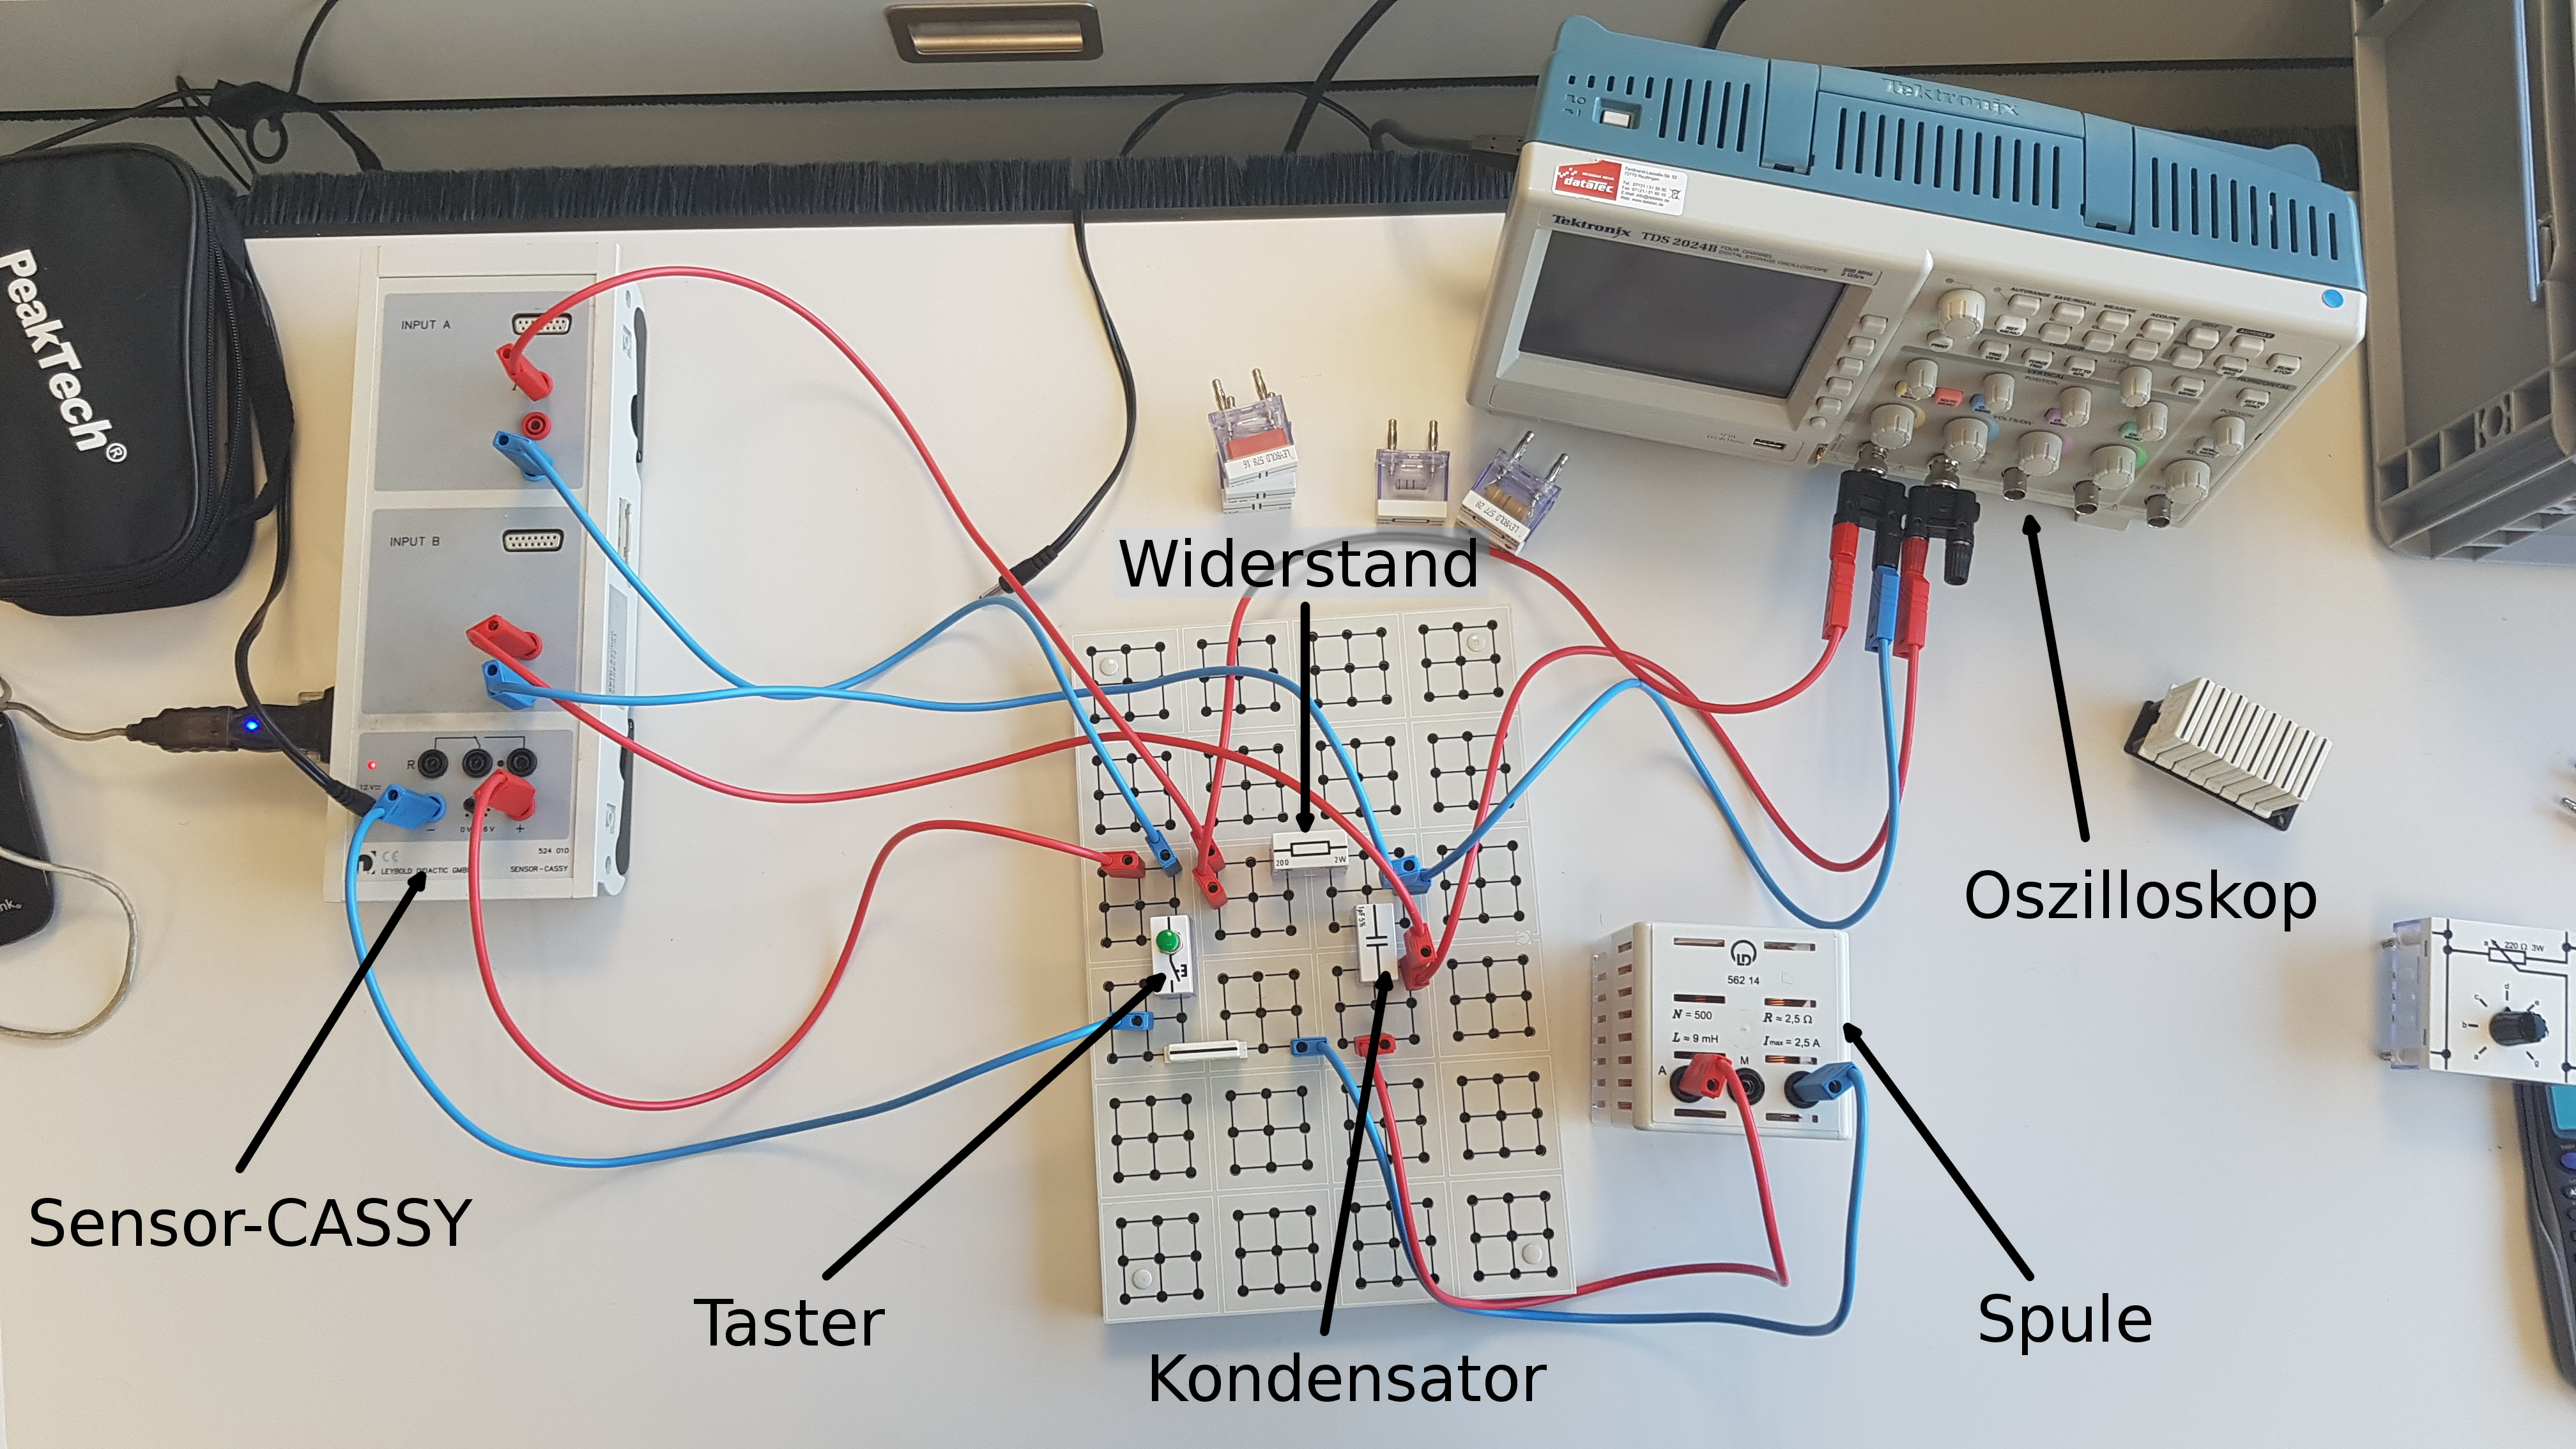
\includegraphics[width=\textwidth]{bilder/LCR_aufbau_beschriftet.jpg}
\caption{Versuchsaufbau LCR-Schwingkreis}
\label{abb:aufbau_lcr}
\end{figure}
Das Schaltbild aus Abbildung \ref{abb:schaltLCR} wird auf der Rastersteckplatte aufgebaut. Dies ist in Abbildung \ref{abb:aufbau_lcr} zu sehen. Als Spannungsquelle dient die Spannungsquelle des Sensor-CASSY. Die Spannung am Kondensator wird am Eingang B und die Stromstärke am Eingang A gemessen. Zusätzlich wird die Spannung am Kondensator am Channel 1 und die Spannung am Widerstand am Channel 2 des Oszilloskops gemessen. Die Erde liegt dabei zwischen Kondensator und Widerstand.

\subsection{Versuchsdurchführung}

Die Schwingungen werden im Modus \glqq automatische Aufnahme\grqq{} mit folgenden Messparametern aufgenommen:
\begin{enumerate}[-]
\item Messbereich Strom $I$: $\pm 0.3$A
\item Messbereich Spannung am Kondensator $U_C$: $\pm 10V$
\item Messintervall: $10\mu\text{s}$
\item Anzahl an Messpunkten: $2000$
\item Messzeit: $20$ms
\end{enumerate}
Um möglich direkt nach Betätigung des Tasters die Aufnahme zu beginnen, wird ein Trigger verwendet. Dieser aktiviert die Messung bei einer steigenden Flanke von $U_C$, die den Schwellenwert von $-9.2$V überschreitet. Das ist sinnvoll, weil die Spannungsquelle auf $U_0 = 9.4$V eingestellt ist und die Polung des Messgerätes zu einer gemessenen Kondensatorspannung von $-9.4$V bei offenem Taster führt. 
Vorab werden die im Versuch verwendeten Widerstände mit Hilfe eines Multimeters auf ihren tatsächlichen Widerstandswert geprüft. In Tabelle \tef{tab:widerstaende} sind die verwendeten Widerstände mit Herstellerangabe und gemessenen Werten angegeben.

\begin{table}[H]
\centering
\begin{tabular}{c|c}
Herstellerangabe / $\Omega$ & Gemessener Wert / $\Omega$ \\
\hline
$1$ & $1.008 \pm 0.001$ \\
$5.1$ & $5.101 \pm 0.001$ \\
$10$ & $9.990 \pm 0.002$ \\
$20$ & $19.82 \pm 0.01$ \\
$47$ & $46.67 \pm 0.01$ \\
$100$ & $99.24 \pm 0.04$ \\
$1000$ & $991.20\pm 0.08$
\end{tabular}
\caption{Herstellerangaben für die verwendeten Widerstände und deren mittels Multimeter gemessene Widerstandswerte samt Fehler.}
\label{tab:widerstaende}
\end{table}
Die nun folgenden Rechnungen verwenden die gemessenen Widerstandswerte. Zusätzlich werden drei in Reihe geschaltete $1\text{k}\Omega$ Widerstädnde verwendet, um einen Widerstand von $3\text{k}\Ohm$ zu erreichen. Da diese Messung jedoch nur zur Visualisierung des Kriechsfalls dient, wird kein genauer Wert benötigt. 

\subsection{Versuchsauswertung}

Beispielhafte Rohdaten für alle verschiedenen Fälle sind in Abbildung \ref{abb:rohdaten_ska} zu sehen.

\begin{figure}[H]
\centering
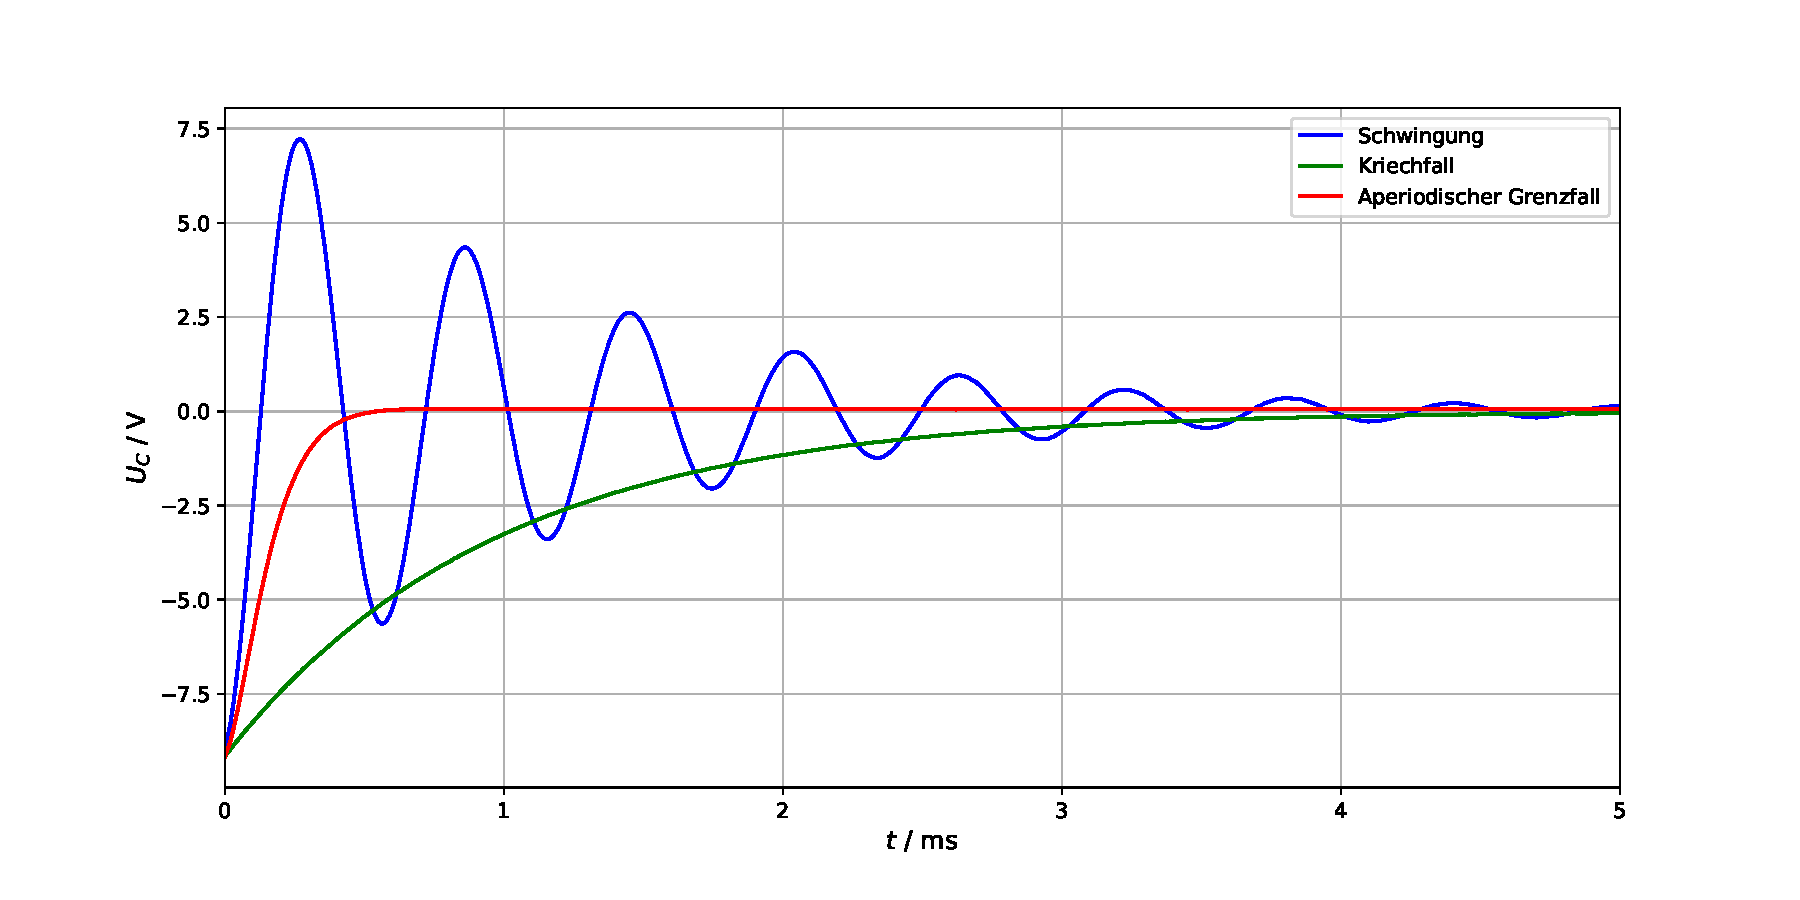
\includegraphics[width=\textwidth]{plots/rohdaten_ska.pdf}
\caption{Rohdaten mit Schwing-, Kriech- und Aperiodischem Grenzfall}
\label{abb:rohdaten_ska}
\end{figure}

\subsubsection{Schwingfall}
Zunächst bestimmen wir die Frequenzen und die Dämpfungen der aufgenommenen Schwingungen für die verschiedenen verwendeten Ohmschen Widerstände. Um die Frequenz bzw. die Periodendauer zu bestimmen, existieren zwei Möglichkeiten. Einerseits ist die Analyse mittels FFT möglich. Andererseits können die Extrema aus den Rohdaten abgelesen und die Periodendauer mittels Regression über die Schwingungsanzahl bestimmt werden.
Analog dazu besteht die Möglichkeit, die Dämpfung $\delta$ aus Gleichung \ref{eq:i_lsg} durch logarithmisches Auftragen der Extrema, d.h. mit Regression, zu berechnen: Es gilt
$$sin(\omega t_i) = \pm 1$$
für die Zeitpunkte $t_i$ an denen $I$ bzw. $U_C$ ein Extremum annimmt. Durch logarithmieren der Gleichung \ref{eq:i_lsg} erhält man für diese Zeiten $t_i$ dann
$$\log \lvert I(t_i)\rvert = -\delta t_i + \log\left\lvert CU_0 \left(\omega+\frac{\delta^2}{\omega}\right)\right\rvert$$
beziehungsweise eine analoge Form für $U_C$. Natürlich kann $\delta$ durch die Verwendung eines Steigungsdreiecks auch nur bei zwei ablesbaren Maxima oder Minima bestimmt werden:
$$\delta = \frac{\log\left(\frac{U_C(t_0)}{U_C(t_1)}\right)}{t_1-t_0}$$
Bei beiden Vorgehensweisen muss der Offset korrigiert werden. Als zweite Option für die Berechnung von $\delta$ kann eine Exponentialfunktion als Einhüllende gefittet werden und die Dämpfung $\delta$ aus dem Fit abgelesen werden.
Für den $100\Omega$ Widerstand sind Regressionen nicht praktikabel, da - aufgrund der starken Dämpfung - zu wenige Extrema genau ablesbar sind. Ein beispielhaftes Ergebnis für die Regression von abgelesenen Extrema bei der Schwingung des $10\Omega$ Widerstand ist in Abbildung \ref{abb:reg1} dargestellt. Die übrigen durchgeführten Regressionen sind im Anhang \ref{app:reg} abgebildet.

\begin{figure}[h]
\centering
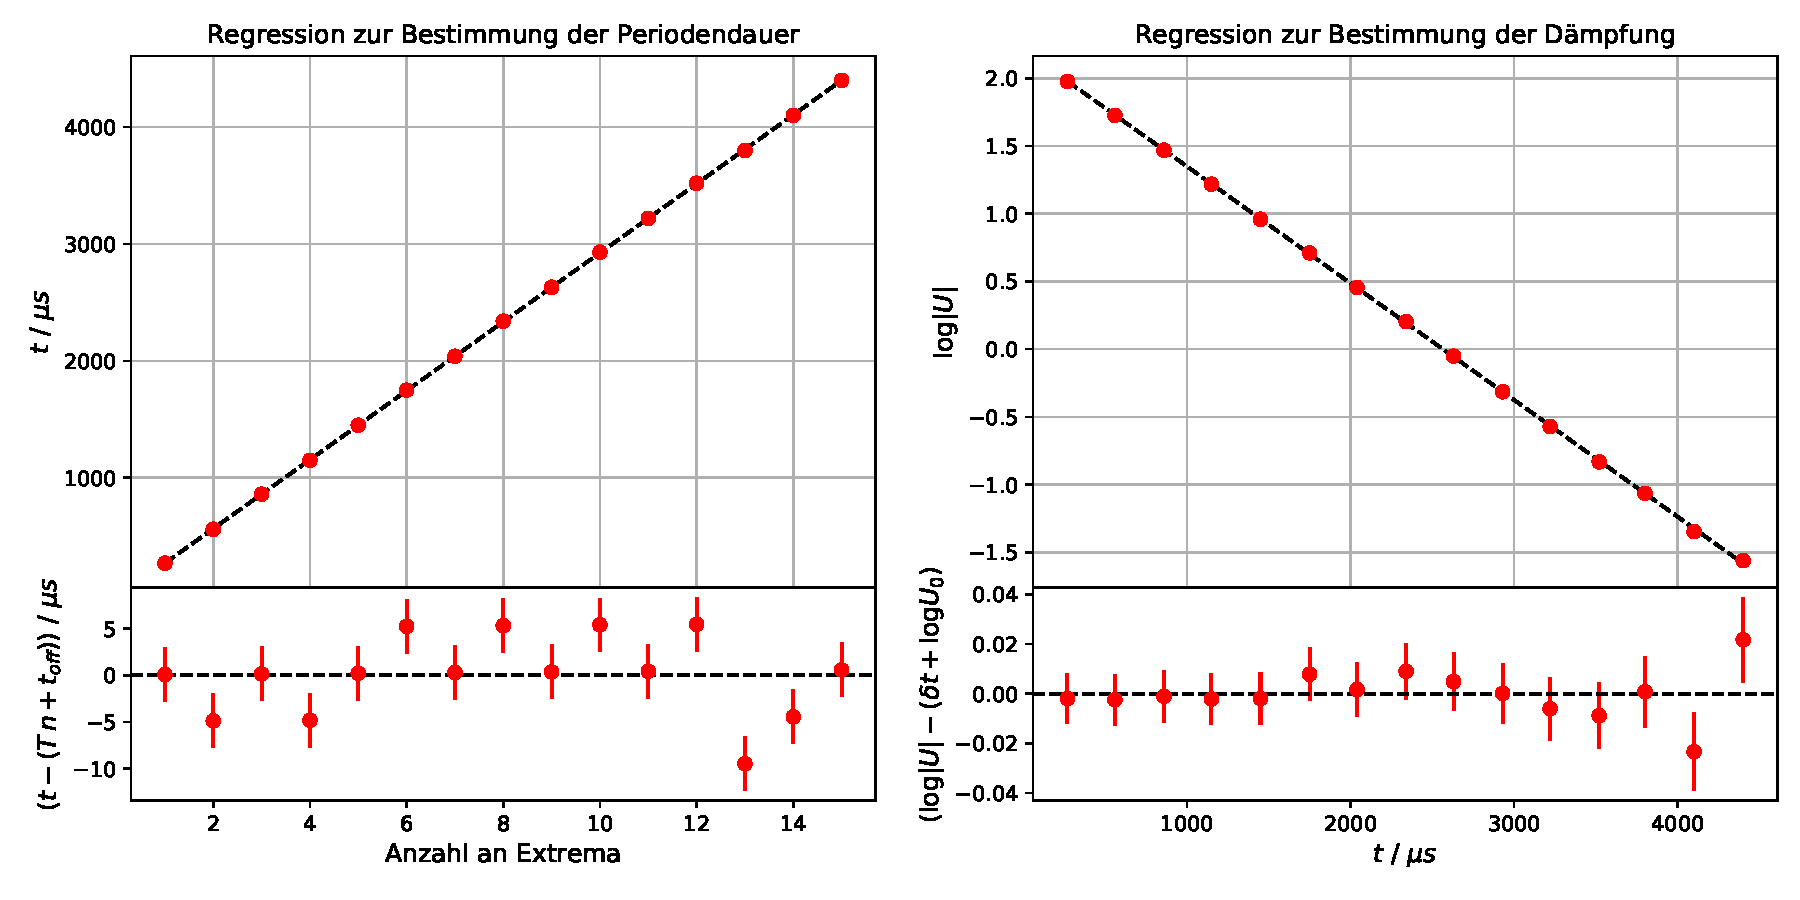
\includegraphics[width=\textwidth]{plots/reg_schwingung3.pdf}
\caption{Regressionen für den $10\Omega$ Widerstand zur Bestimmung von $\frac{T}{2}$ und $\delta$.}
\label{abb:reg1}
\end{figure}

\begin{figure}[h]
\centering
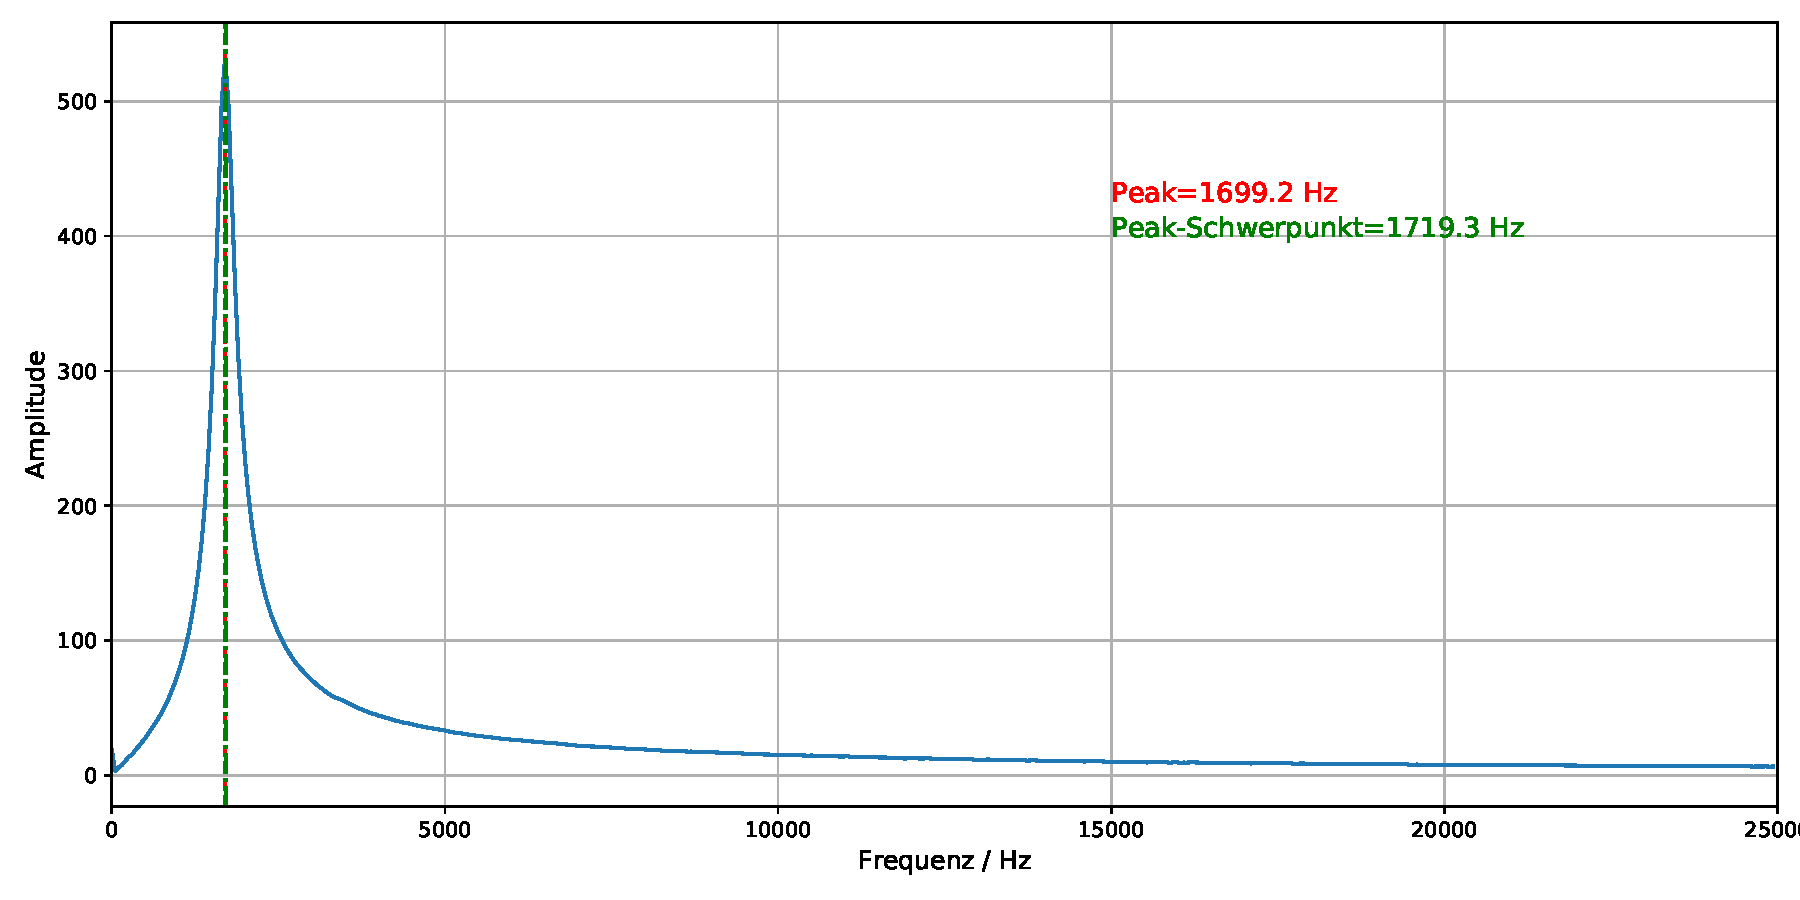
\includegraphics[width=\textwidth]{plots/fft/fft_schwingung3_1.pdf}
\caption{Mittels FFT berechnetes Spektrum für die erste Messung des $10\Omega$ Widerstands. Die rote Linie zeigt das Argument-Maximum an. Die grüne Linie Hingegen den Peak-Schwerpunkt.}
\label{abb:fft1}
\end{figure}

Für die Frequenzen ergeben sich die in Tabelle \ref{tab:freq} dargestellten Werte. Die FFT-Werte stammen aus der Peakfinder-Methode. Dabei sollte man beachten, dass der FFT-Algorithmus die Frequenz mit einer Breite von $h\approx 49.975 \text{Hz}$ diskretisiert. Dies mindert die Qualität der Methode. Als Fehler der Einzelmessungen wurde die Differenz aus Argument-Maximum der Amplitude und Peak-Schwerpunkt verwendet. Der Fehler des gewichteten Mittels ist der innere Fehler der Einzelmessungen. Das Frequenzspektrum der ersten Messung des $10\Omega$ Widerstands ist in Abbildung \ref{abb:fft1} zu sehen. Für die übrigen Widerstände befindet sich jeweils das Spektrum der 1. Messung im Anhang \ref{app:fft}.

\begin{table}[H]
\centering
\begin{adjustbox}{width=\textwidth}
\begin{tabular}{c|c|cccc}
\multirow{2}{*}{Ohmscher Widerstand / $\Omega$} & \multirow{2}{*}{Regression / Hz} & \multicolumn{4}{c}{FFT / Hz} \\
\cline{3-6}
& & Messung 1 & Messung 2 & Messung 3 & Mittel\\
\hline
$1$ & $1696.9 \pm 0.6$ & $1715.7\pm 16.6$ & $1715.2\pm 16.1$ & $1715.3\pm 16.1$ & $1715.4\pm 9.4$\\
$5.1$ & $1696.3 \pm 0.7$ & $1718.9\pm 19.7$ & $1719.0\pm 19.8$ & $1719.0\pm 19.8$ & $1718.9\pm 11.4$\\
$10$ & $1695.1 \pm 1.0$ & $1719.3\pm 20.1$ & $1719.3\pm 20.1$ & $1719.2\pm 20.0$ & $1719.2\pm 11.6$ \\
$20$ & $1689.2 \pm 2.1$ & $1720.4\pm 21.3$ & $1720.3\pm 21.2$ & $1720.3\pm 21.2$ & $1720.4\pm 12.2$\\
$47$ & $1628.6 \pm 4.8$ & $1761.1\pm 62.0$ & $1761.3\pm 62.1$ & $1741.5\pm 42.4$ & $1751.0 \pm 30.5$\\
$100$ & - & $1294.7\pm 154.6$ & $1293.4\pm 155.8$ & $1339.0\pm 110.3$ & $1316.4 \pm 77.8$
\end{tabular}
\end{adjustbox}
\caption{Mit Regression und FFT ermittelte Frequenzwerte.}
\label{tab:freq}
\end{table}

Die Messungen des $100\Omega$ Widerstands werden von nun an nicht weiter ausgewertet, da die kurze Schwingzeit keine zuverlässigen Ergebnisse ermöglicht. Desweiteren arbeitet die Peakfinder-Methode wegen der groben Diskretisierung der Frequenz durch den FFT-Algorithmus nicht korrekt, sodass die Frequenzen der Regressionsmethode als weitere Berechnungsgrundlage dienen. Ein Indiz dafür, dass die Frequenzwerte aus dem Spektrum systematisch fehlerhaft sind, ist, dass sie mit steigendem Widerstand steigen, obwohl
$$\omega^2 = \omega_0^2 + \delta^2$$
mit der korrigierten Frequenz $\omega_0$ und der Dämpfung $\delta$ gilt und sie daher, wie die Regressionsdaten, fallen müssten. Folgende Dämpfungswerte wurden berechnet:

\begin{table}[H]
\centering
\begin{tabular}{c|c}
Herstellerangabe / $\Omega$ & Dämpfung / Hz \\
\hline
$1$ & \\
$5.1$ & \\
$10$ &  \\
$20$ & \\
$47$ & \\
$100$ & 
\end{tabular}
\end{table}

\subsubsection{Aperiodischer Grenzfall}

\subsubsection{Kriechfall}



\subsection{Fazit}




\section{Gekoppelte LC-Schwingkreise}


\subsection{Versuchsbeschreibung}

In diesem Versuch werden zwei Schwingkreise induktiv miteinander gekoppelt. Speziell werden hier die beiden Fundamentalschwingungen bei gleichsinniger und gegensinniger Anregung und eine Schwebung aufgezeichnet.

\begin{figure}[H]
\centering
\begin{tikzpicture}
% Linke Schwingkreise
\draw (0,0.2) -- (-1,0.2) to [rmeterwa, t=$U_1$] (-1,1.8) -- (0,1.8);
\draw (0.8,0) node[ocirc]{} -- (0,0) to [C, a=$C$] (0,2) -- (2,2) to [cute inductor, a=$L$] (2,0) -- (1.2,0) node[ocirc]{};
\draw (3.55,0) node[ocirc]{} -- (2.75,0) to [cute inductor, a=$L$] (2.75,2) -- (4.75,2) to[C, a=$C$] (4.75,0) -- (3.95,0) node[ocirc]{};
\draw (4.75,0.2) -- (5.75,0.2) to [rmeterwa, t=$U_2$] (5.75,1.8) -- (4.75,1.8);
\draw (2,0) to [normal open switch] (2,-1) -- (0,-1) -- (0,0);
\draw (2.75,0) to [normal open switch] (2.75,-1) -- (4.75,-1) -- (4.75,0);
\draw[dashed, thin] (2.15,-0.5) -- (2.85,-0.5); 


% Rechte Schwingkreise
\draw (8,0.2) -- (7,0.2) to [rmeterwa, t=$U_1$] (7,1.8) -- (8,1.8);
\draw (8.8,0) node[ocirc]{} -- (8,0) to [C, a=$C$] (8,2) -- (10,2) to [cute inductor, a=$L$] (10,0) -- (9.2,0) node[ocirc]{};
\draw (11.55,0) node[ocirc]{} -- (10.75,0) to [cute inductor, a=$L$] (10.75,2) -- (12.75,2) to[C, a=$C$] (12.75,0) -- (11.95,0) node[ocirc]{};
\draw (12.75,0.2) -- (13.75,0.2) to [rmeterwa, t=$U_2$] (13.75,1.8) -- (12.75,1.8);
\draw (10,0) to [normal open switch] (10,-1) -- (8,-1) -- (8,0);
\draw (10.75,0) to [normal open switch] (10.75,-1) -- (12.75,-1) -- (12.75,0);
\draw[dashed, thin] (10.15,-0.5) -- (10.85,-0.5); 

\end{tikzpicture}
\caption{Fundamentalschwingungen der gekoppelten Schwingkreise bei gleichsinniger (links) und gegensinniger Anregung (rechts)}
\end{figure}

Bei überbrückter Spannungsquelle gelten für den gekoppelten Schwingkreis die folgenden Differentialgleichungen 
\begin{align*}
\ddot I_1 + k \ddot I_2 + \frac{1}{LC}I_1 &= 0 \\
\ddot I_2 + k \ddot I_1 + \frac{1}{LC}I_2 &= 0
\end{align*}
Dabei bezeichnet $k \in (0,1)$ die Kopplung der beiden Schwingkreise. 
Mit den sogenannten \textit{Fundamentalströmen} $I_+ = I_1 + I_2$ und $I_- = I_1 - I_2$ erhält man durch Addition bzw. Subtraktion der obigen Gleichungen und anschließendem Umformen
\begin{align*}
\ddot I_+ + \frac{1}{LC(1+k)} I_+ = 0 \\
\ddot I_- + \frac{1}{LC(1-k)} I_- = 0
\end{align*}
Daraus ergeben sich harmonische Schwingungen mit den Kreisfrequenzen 
$$\omega_+ = \frac{\omega_0}{\sqrt{1+k}} \hspace{0.2cm} \text{ und } \hspace{0.2cm} \omega_- = \frac{\omega_0}{\sqrt{1+k}}.$$
Dabei ist $\omega_0 = \frac{1}{\sqrt{LC}}$ die Kreisfrequenz der ungekoppelten Schwingung. Mithilfe der Fundamentalschwingungen lässt sich dann der Kopplungsgrad bestimmen
$$k = \frac{f_-^2 - f_+^2}{f_-^2 + f_+^2}.$$
Bei Messung einer Schwebung mit Schwebungsfrequenz $f_s$ und Frequenz der gekoppelten Schwingung $f_k$ kann man die Fundamentalschwingungen gemäß
$$f_k = \frac{f_- + f_+}{2} \hspace{0.2cm} \text{ und } \hspace{0.2cm} f_s = \frac{f_- - f_+}{2}$$
bestimmen. Aufgrund der unvermeidbaren Dämpfung der beiden Schwingkreise sind die Extrema des einen Schwingkreises gegen die Nulldurchgänge des anderen verschoben. Für Kopplungen $k < 0.2$ gilt näherungsweise für die zeitliche Verschiebung
$$\Delta t \approx \frac{1}{\omega_s} \left( \frac{\pi}{2} - \arctan\left(  \frac kR \sqrt{\frac LC}\right) \right).$$


\subsection{Versuchsaufbau}

\subsection{Versuchsdurchführung}

\subsection{Versuchsauswertung}

\subsection{Fazit}

\newpage
\appendix
\section{LCR-Schwingfall: Regressionen der übrigen Widerstände}\label{app:reg}
\begin{figure}[H]
\centering
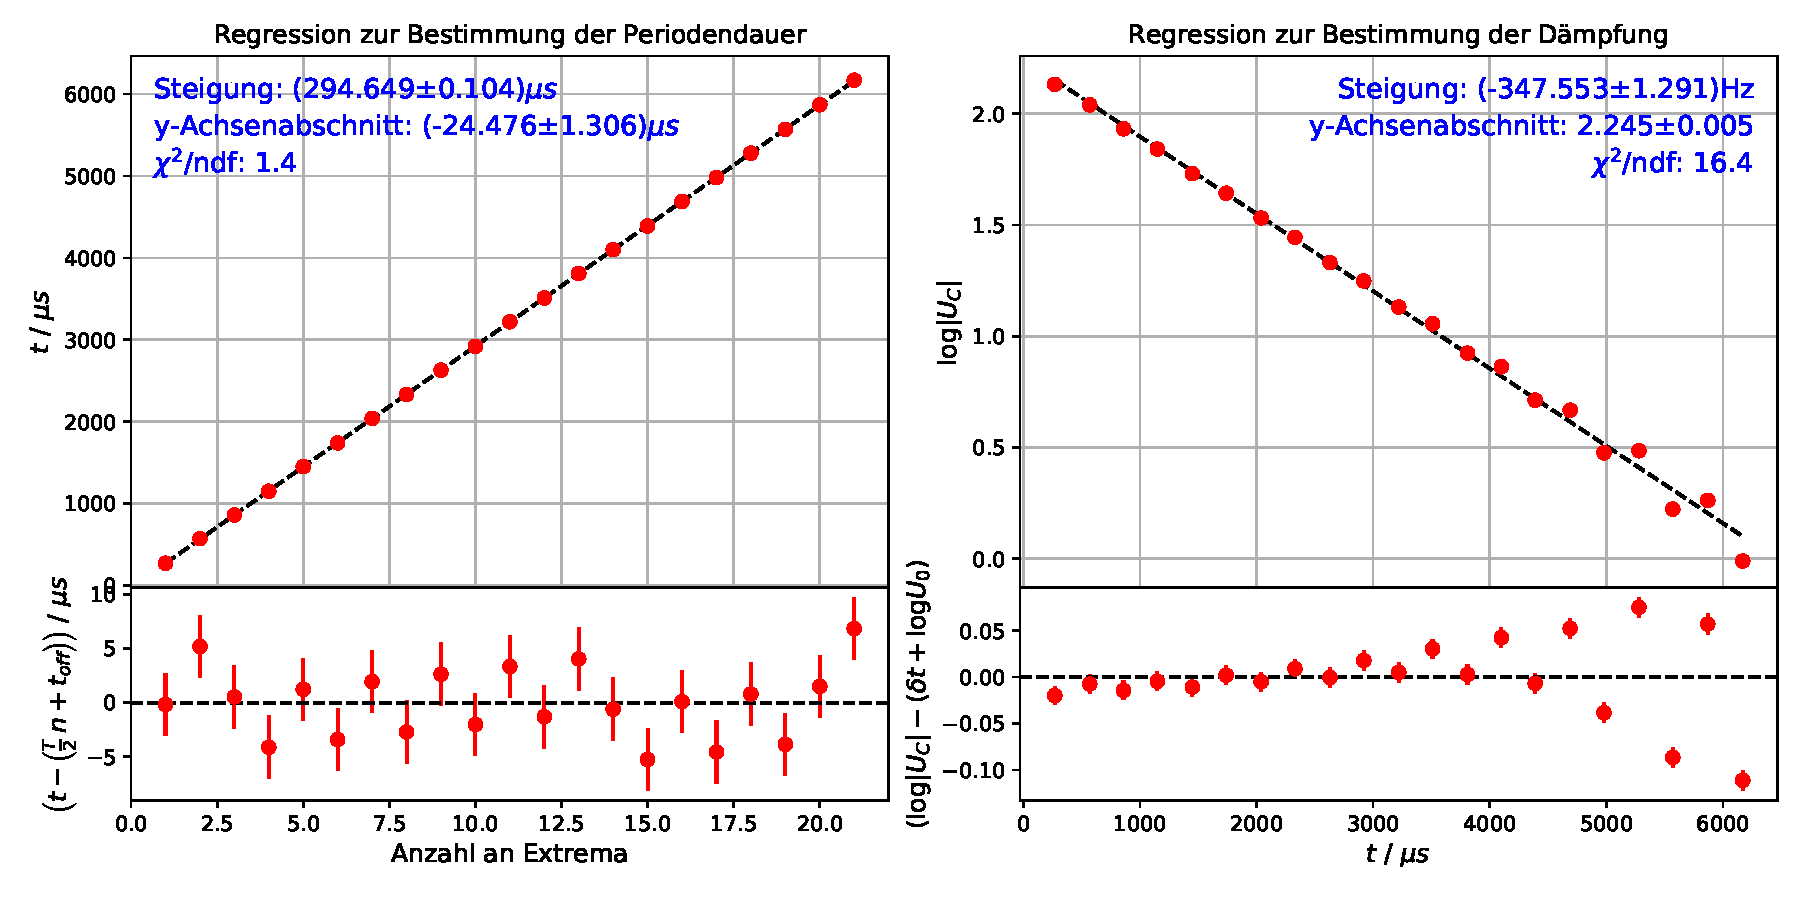
\includegraphics[width=\textwidth]{plots/reg_schwingung1.pdf}
\caption{Regressionen für den $1\Omega$ Widerstand zur Bestimmung von $\frac{T}{2}$ und $\delta$}
\end{figure}
\begin{figure}[H]
\centering
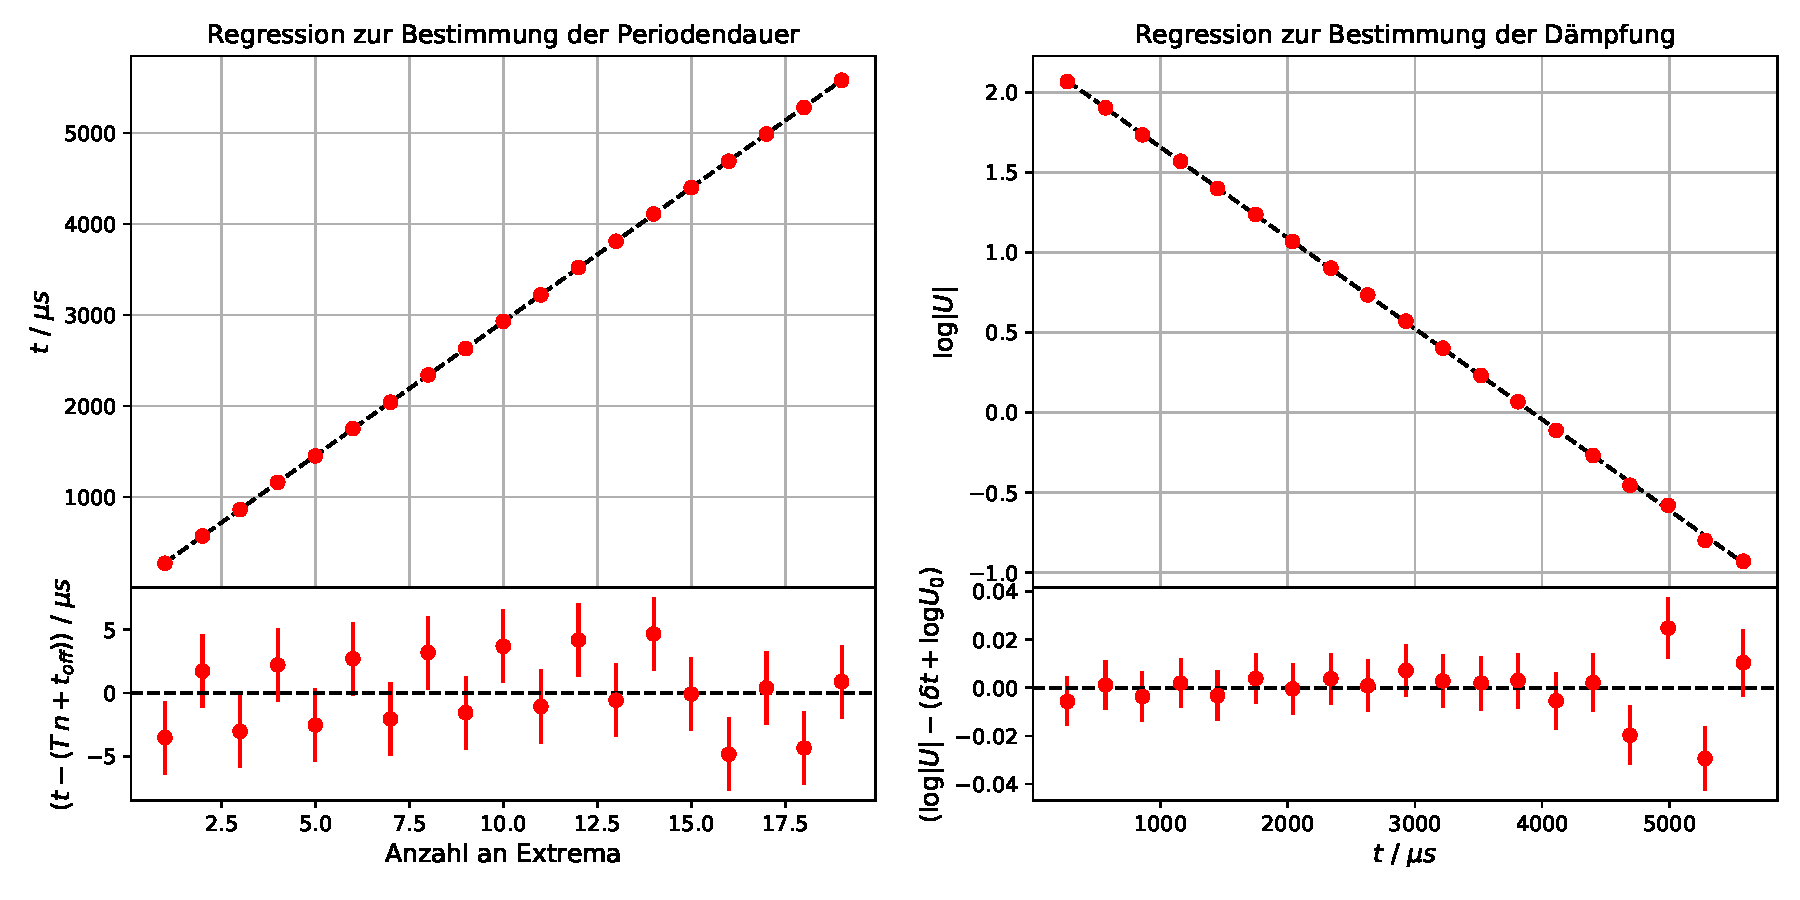
\includegraphics[width=\textwidth]{plots/reg_schwingung2.pdf}
\caption{Regressionen für den $5.1\Omega$ Widerstand zur Bestimmung von $\frac{T}{2}$ und $\delta$}
\end{figure}
\begin{figure}[H]
\centering
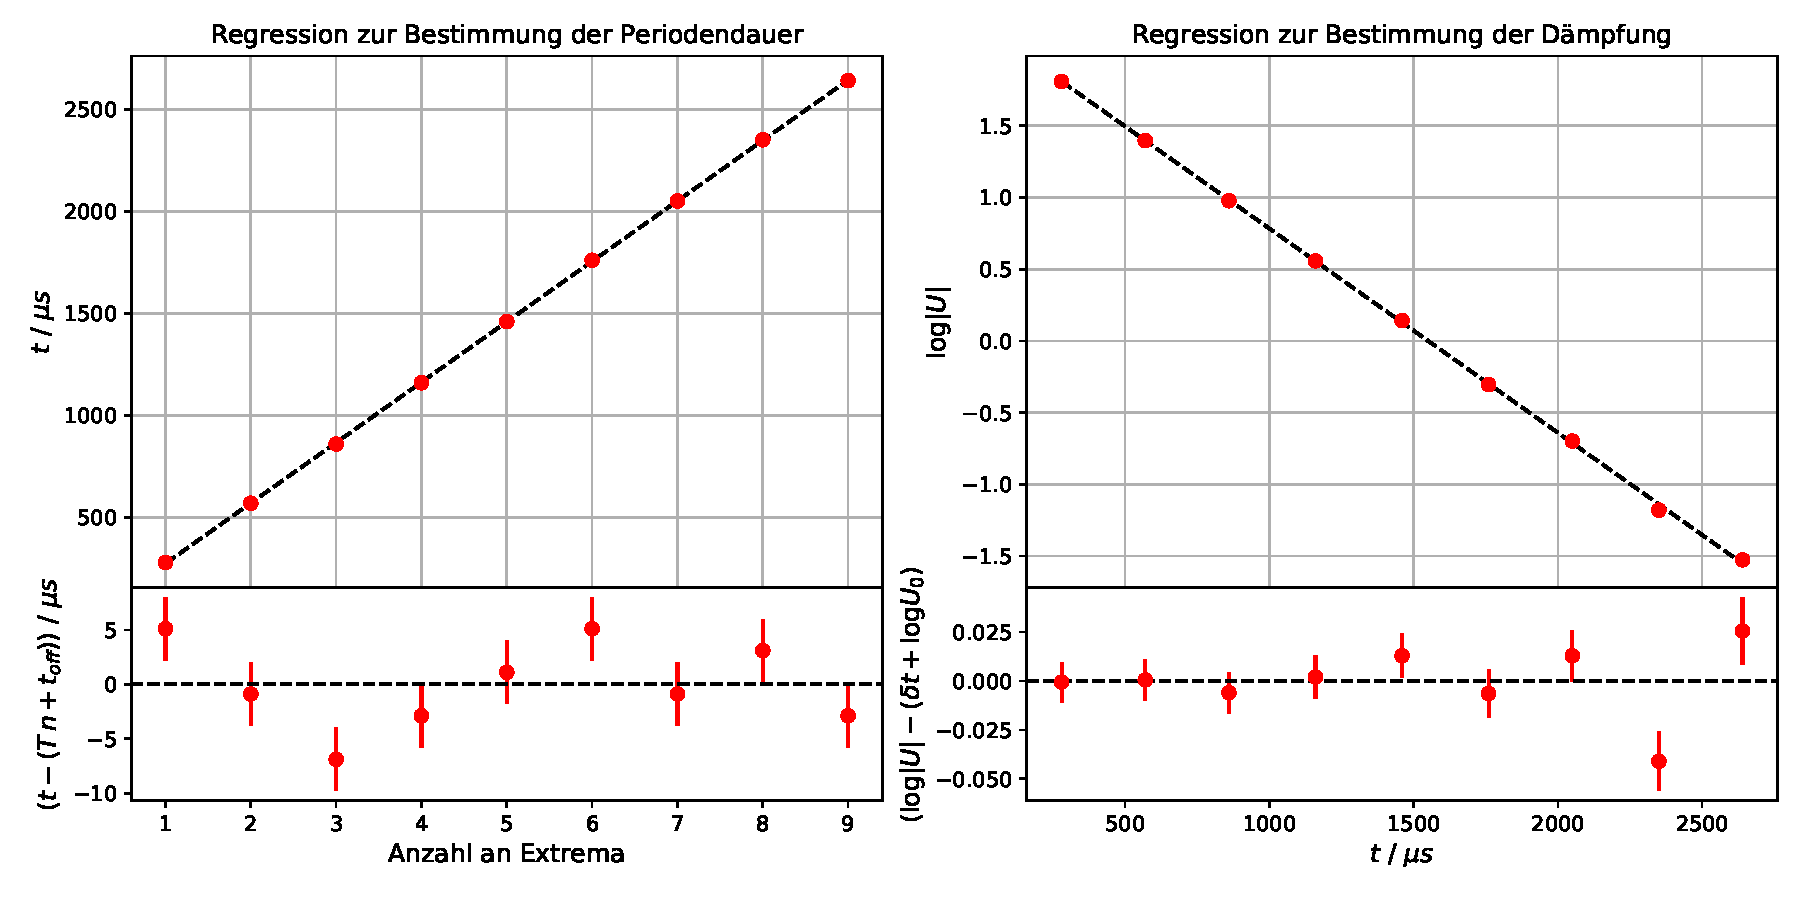
\includegraphics[width=\textwidth]{plots/reg_schwingung4.pdf}
\caption{Regressionen für den $20\Omega$ Widerstand zur Bestimmung von $\frac{T}{2}$ und $\delta$}
\end{figure}
\begin{figure}[H]
\centering
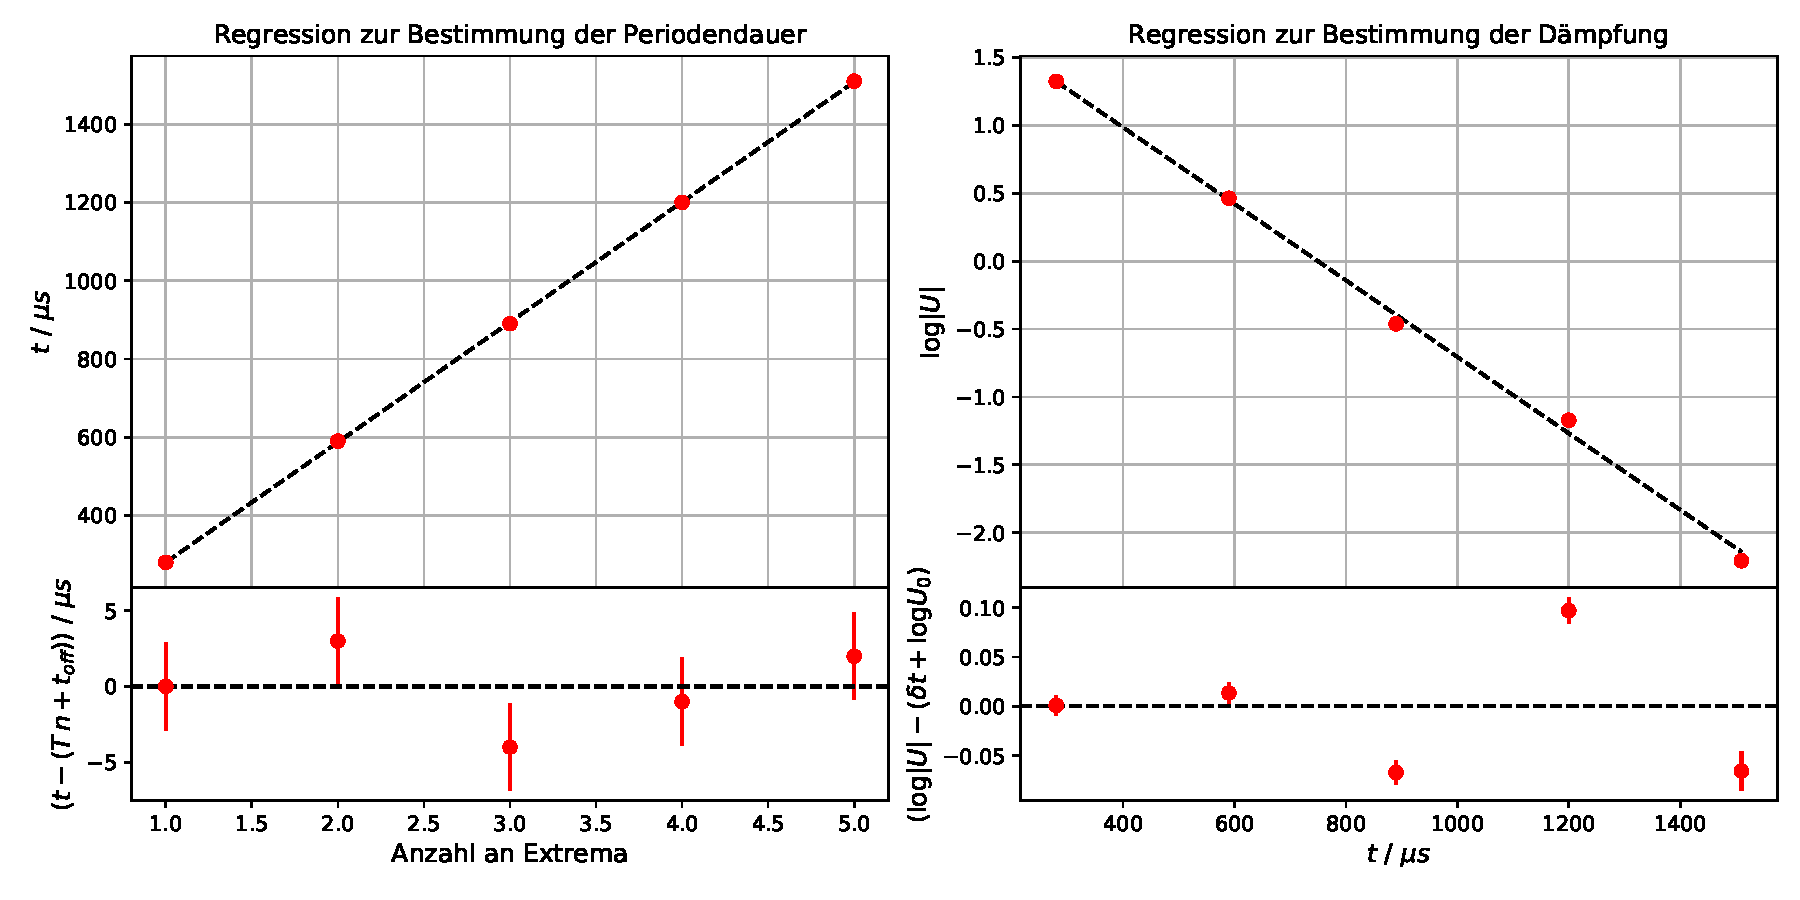
\includegraphics[width=\textwidth]{plots/reg_schwingung5.pdf}
\caption{Regressionen für den $47\Omega$ Widerstand zur Bestimmung von $\frac{T}{2}$ und $\delta$}
\end{figure}
\section{LCR-Schwingfall: FFT der übrigen Widerstände}\label{app:fft}
\begin{figure}[H]
\centering
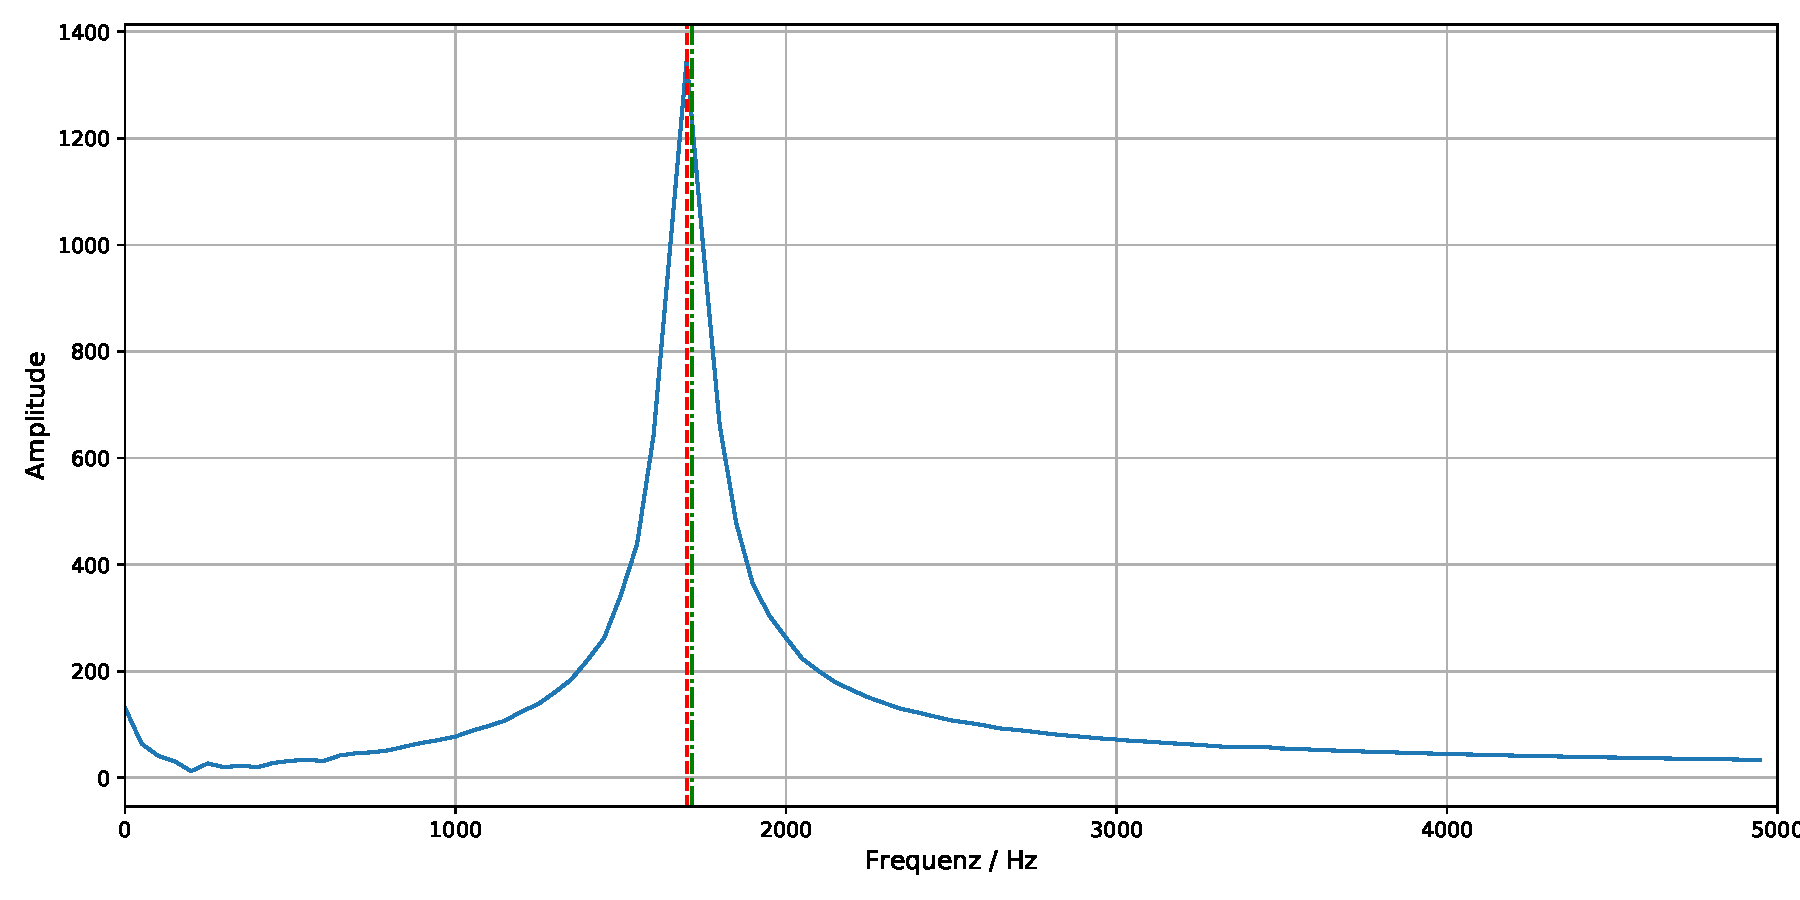
\includegraphics[width=\textwidth]{plots/fft/fft_schwingung1_1.pdf}
\caption{Mittels FFT berechnetes Spektrum für die erste Messung des $1\Omega$ Widerstands. Die rote Linie zeigt das Argument-Maximum an. Die grüne Linie Hingegen den Peak-Schwerpunkt.}
\end{figure}
\begin{figure}[H]
\centering
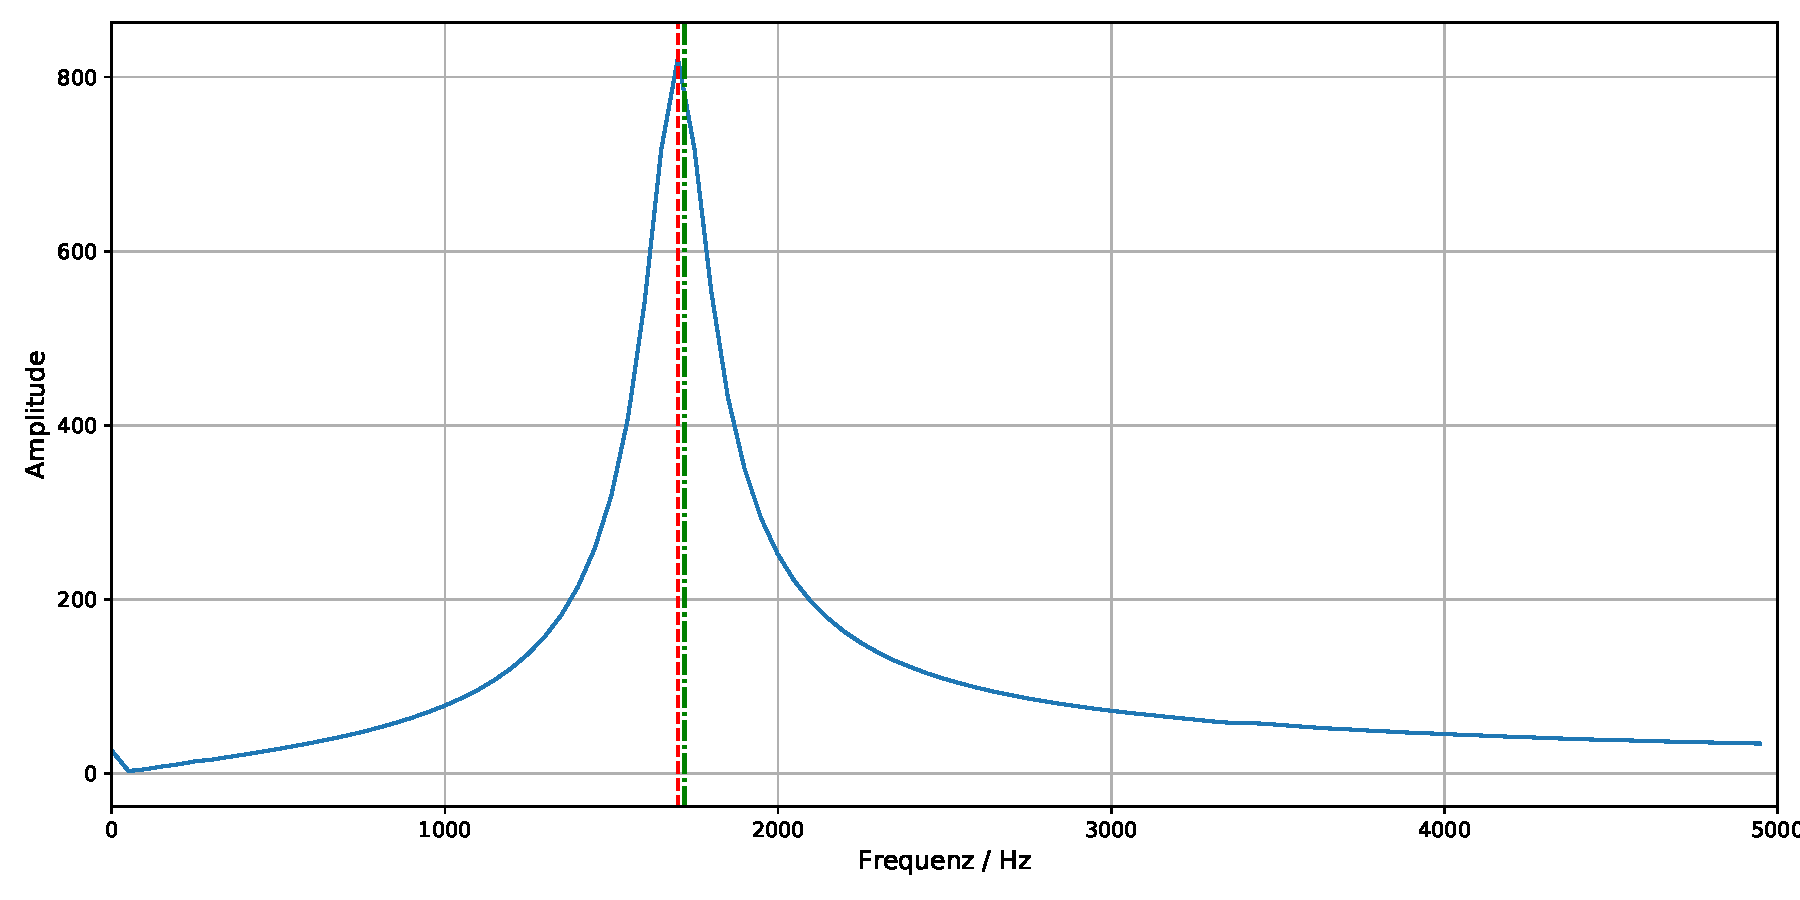
\includegraphics[width=\textwidth]{plots/fft/fft_schwingung2_1.pdf}
\caption{Mittels FFT berechnetes Spektrum für die erste Messung des $5.1\Omega$ Widerstands. Die rote Linie zeigt das Argument-Maximum an. Die grüne Linie Hingegen den Peak-Schwerpunkt.}
\end{figure}
\begin{figure}[H]
\centering
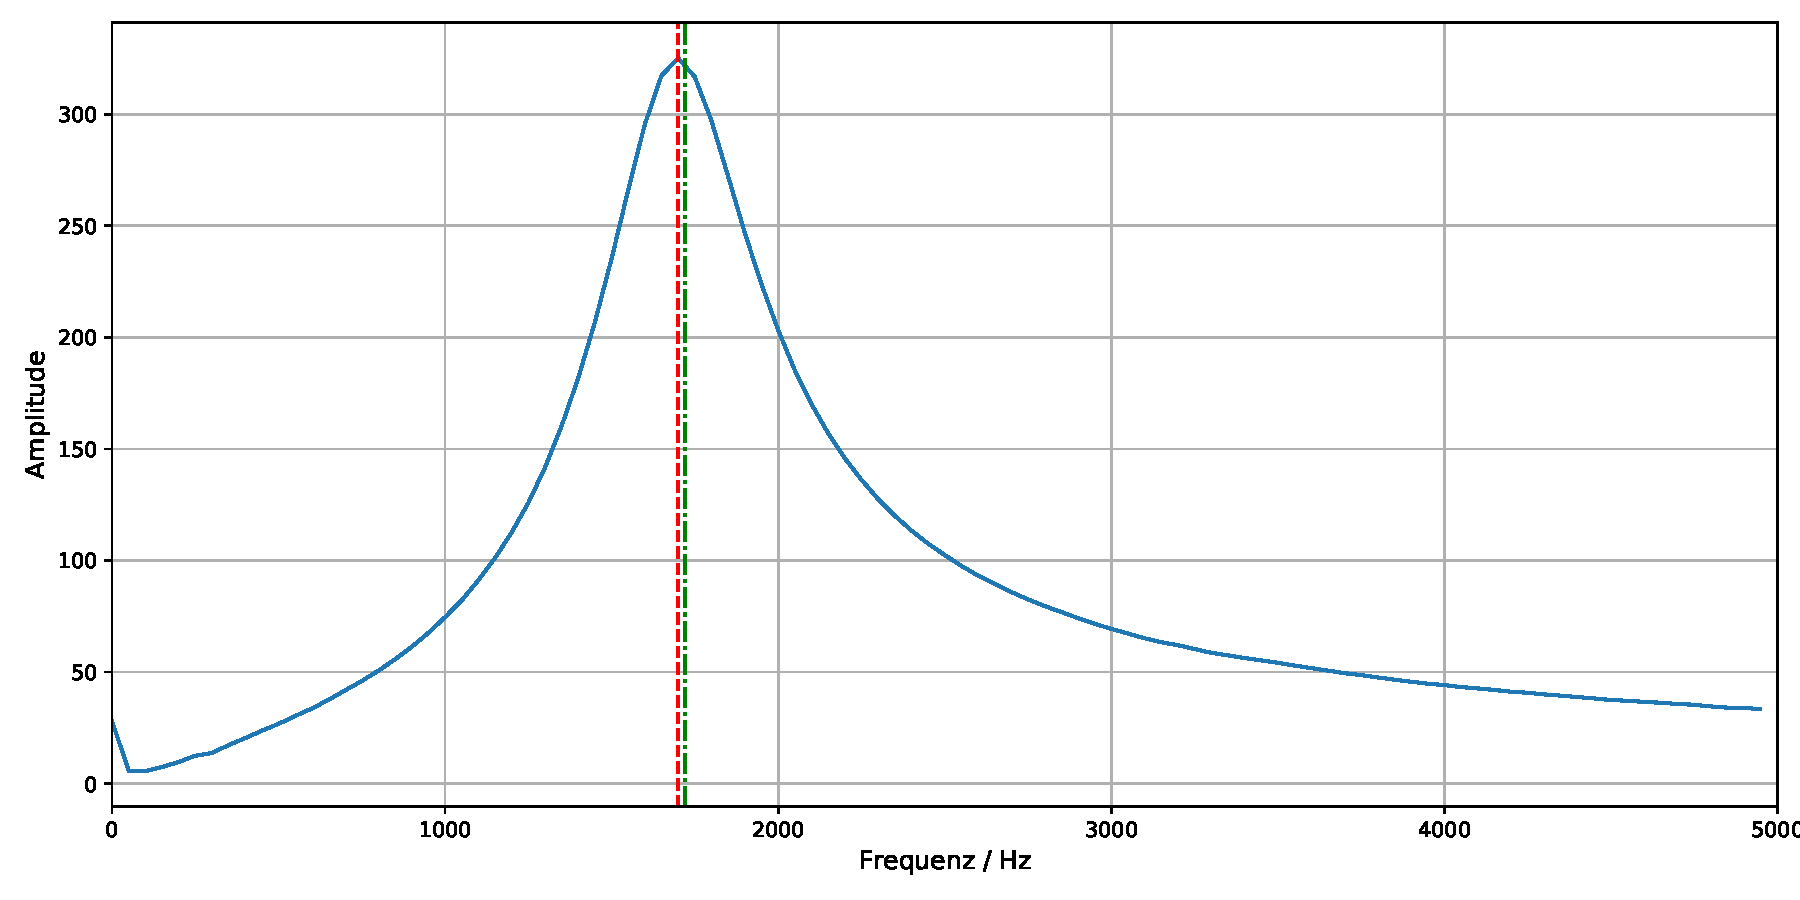
\includegraphics[width=\textwidth]{plots/fft/fft_schwingung4_1.pdf}
\caption{Mittels FFT berechnetes Spektrum für die erste Messung des $20\Omega$ Widerstands. Die rote Linie zeigt das Argument-Maximum an. Die grüne Linie Hingegen den Peak-Schwerpunkt.}
\end{figure}
\begin{figure}[H]
\centering
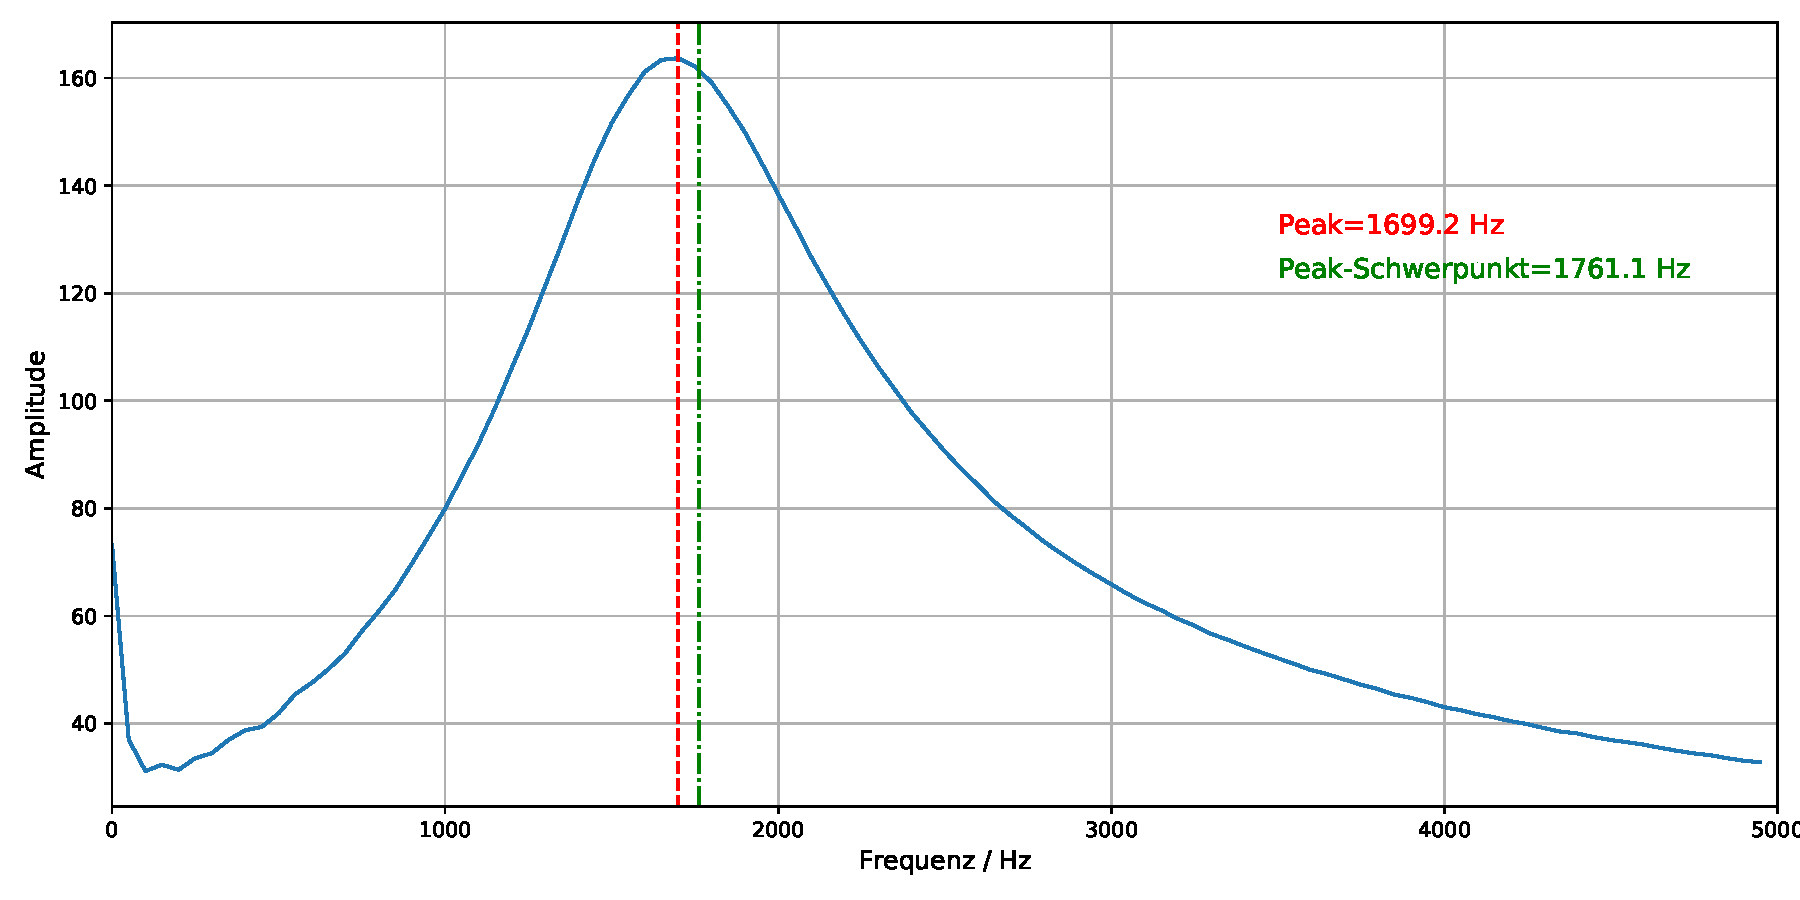
\includegraphics[width=\textwidth]{plots/fft/fft_schwingung5_1.pdf}
\caption{Mittels FFT berechnetes Spektrum für die erste Messung des $47\Omega$ Widerstands. Die rote Linie zeigt das Argument-Maximum an. Die grüne Linie Hingegen den Peak-Schwerpunkt.}
\end{figure}
\begin{figure}[H]
\centering
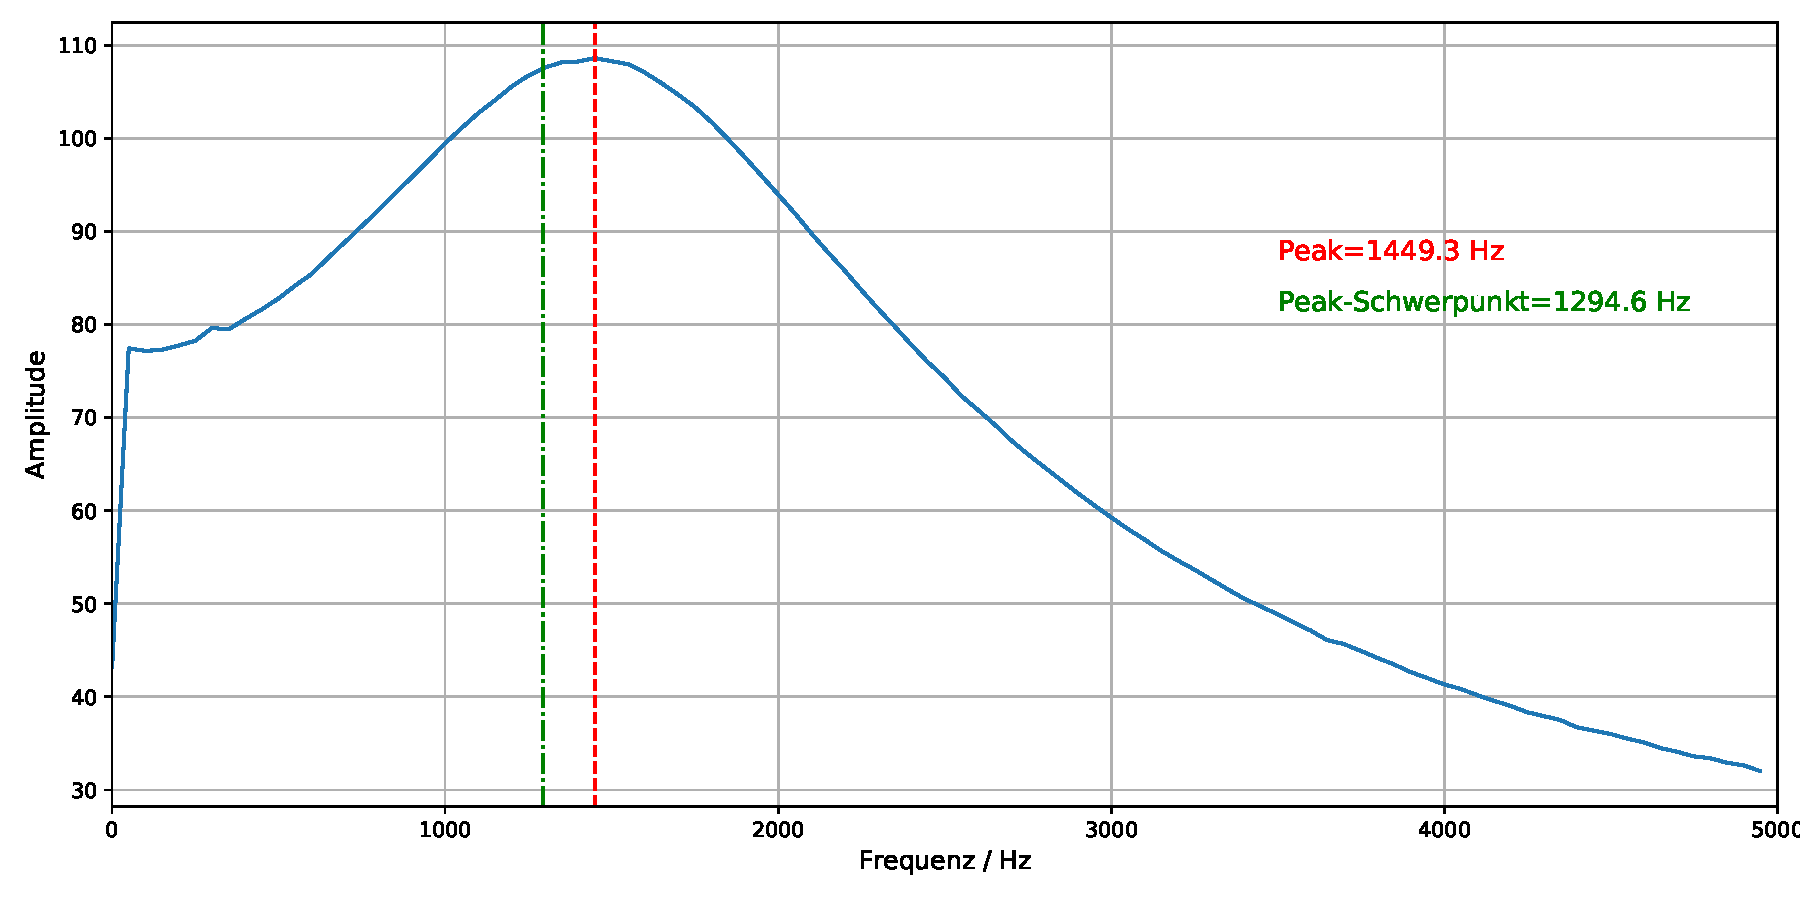
\includegraphics[width=\textwidth]{plots/fft/fft_schwingung6_1.pdf}
\caption{Mittels FFT berechnetes Spektrum für die erste Messung des $100\Omega$ Widerstands. Die rote Linie zeigt das Argument-Maximum an. Die grüne Linie Hingegen den Peak-Schwerpunkt.}
\end{figure}


\end{document}